\documentclass[12pt]{article}
\usepackage[a4paper, margin=1in]{geometry} 
\usepackage{graphicx} 
\usepackage{hyperref}
\usepackage{float}
\usepackage[font=small, labelfont=bf]{caption}

\title{Lecture Notes for \\ INF281 Basics of Bioinformatics Sequence Analysis}
\author{Takaya Saito}
\date{}

\begin{document}

\clearpage\maketitle
\vspace{450px}

\includegraphics[scale=1]{fig00/88x31.png} \\
This work is licensed under a Creative Commons Attribution 4.0 International License.
\thispagestyle{empty}
\pagebreak

\pagenumbering{roman}
\setcounter{page}{1}
\tableofcontents
\pagebreak

\pagenumbering{arabic}
\setcounter{page}{1}

\makeatletter 
\renewcommand{\thefigure}{\arabic{section}.\arabic{figure}}
\makeatother

%
% PART I
%
\part{}

%
% Introduction
%
\setcounter{figure}{0}
\section{Introduction}
%\documentclass[12pt]{article}
%\usepackage[a4paper, margin=1in]{geometry} 
%\usepackage{graphicx} 
%\usepackage{hyperref}
%\usepackage{float}
%\usepackage[font=small, labelfont=bf]{caption}
%
%\begin{document}

%
% Introduction to Molecular Biology
%
\subsection{Introduction to Molecular Biology}
Molecular biology is the study of biology focusing on organisms and cells at the molecular level.

%
% Five essential facts about cells
%
\subsubsection*{Five essential facts about cells}

\textbf{1. Two primary types of cells –- eukaryotes and prokaryotes}
\begin{itemize}
\item Eukaryote: animals \& plants
\item Prokaryote: bacteria \& archaea
\end{itemize}
\begin{figure}[H]
  \centering
      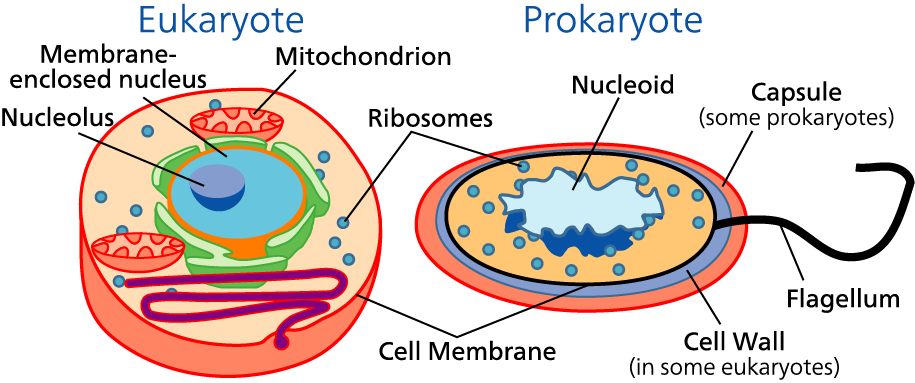
\includegraphics[width=0.75\textwidth]{fig01/prokaryote_and_eukaryote_cells.png}
  \caption{Eukaryotic and prokaryotic cells (source: \href{https://commons.wikimedia.org/wiki/File:Celltypes.svg}{Science Primer, Wikimedia Commons})}
\end{figure}

\noindent \textbf{2. Cell size –- around 1 to 100 micrometers}
\begin{itemize}
\item Cell Size and Scale: \url{http://learn.genetics.utah.edu/content/cells/scale}
\end{itemize}
\medskip  

\noindent \textbf{3. The number of cells}
\begin{itemize}
\item Prokaryotes: 1 cell
\item Human:  Estimate of 15 trillion cells
\end{itemize}
\medskip 

\noindent \textbf{4. An animal cell and cell organelles}
\begin{figure}[H]
  \centering
      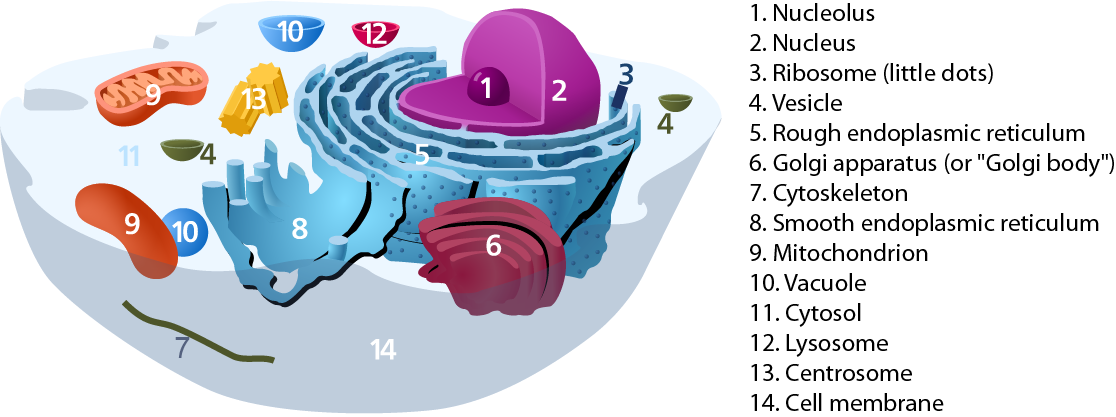
\includegraphics[width=0.75\textwidth]{fig01/animal_cells_and_organelles.png}
  \caption{An animal cell and organelles (source: \href{https://en.wikipedia.org/wiki/Organelle\#/media/File:Animal_Cell.svg}{Kelvinsong, Wikimedia Commons})}
\end{figure}

\noindent \textbf{5. Cellular processes}
\begin{itemize}
\item Cell growth, cell development, cell signaling, …
\item Example: \url{http://www.nature.com/nrg/multimedia/rnai}
\end{itemize}

%
% Central dogma of molecular biology
%
\subsubsection*{Central dogma of molecular biology}

It describes the information flow within a cell.

\begin{figure}[H]
  \centering
      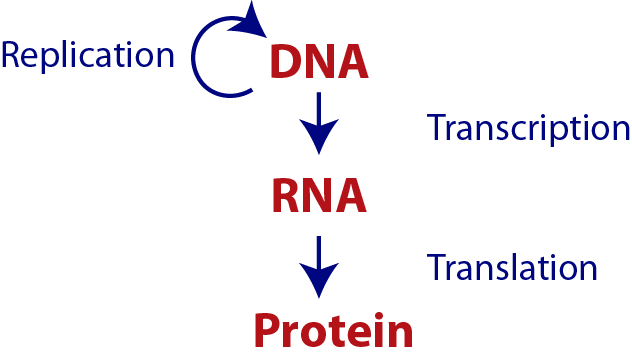
\includegraphics[width=0.75\textwidth]{fig01/central_dogma_of_molecular_biology.png}
  \caption{Central dogma of molecular biology}
\end{figure}

%
% DNA (deoxyribonucleic acid)
%
\subsubsection*{DNA (deoxyribonucleic acid)}

DNA stores genetic information. It has four different bases: cytosine (C), guanine (G), adenine (A), and thymine (T).

\begin{figure}[H]
  \centering
      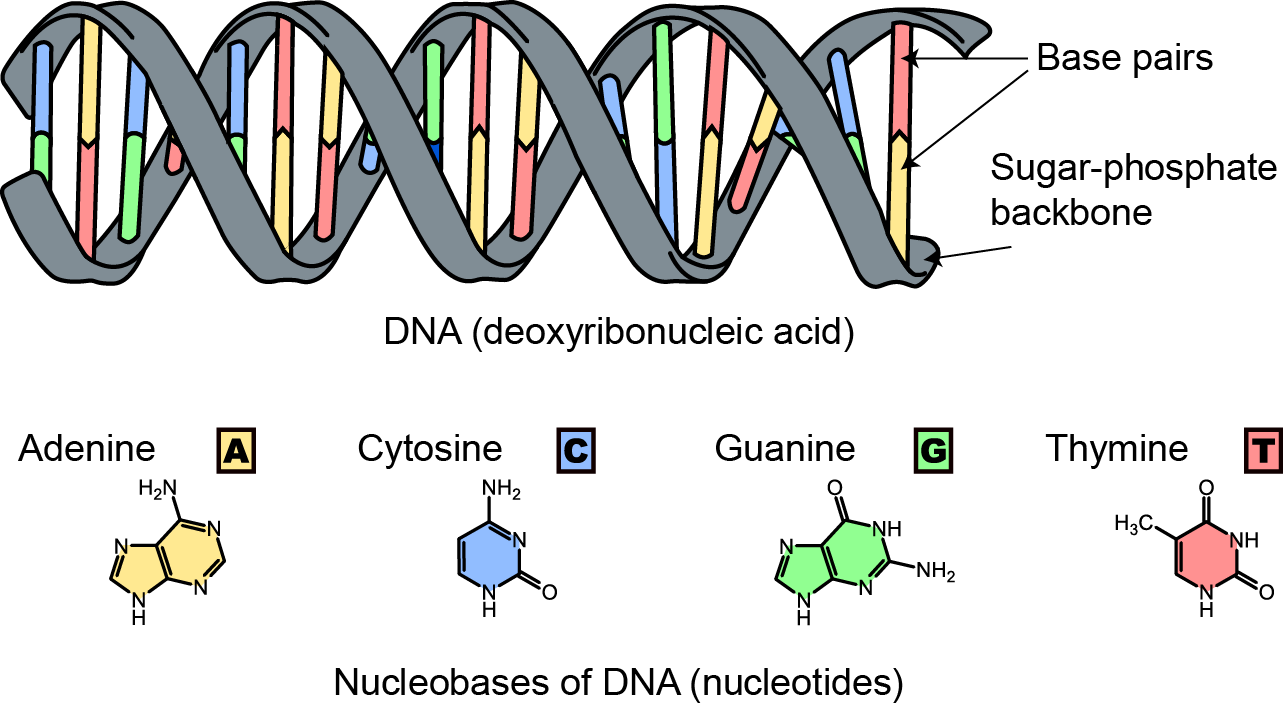
\includegraphics[width=0.5\textwidth]{fig01/dna_bases.png}
  \caption{DNA double helix and base pairs \newline (modified from the original version by \href{https://commons.wikimedia.org/w/index.php?curid=9810855}{Sponk, Wikimedia Commons})}
\end{figure} 

\noindent \textbf{Base pair matching (Watson-Crick base pair)}

\noindent Adenine (A) pairs with thymine (T), whereas cytosine (C) pairs with guanine (G).

\begin{verbatim}
DNA strand1: ACGT
             ||||
DNA strand2: TGCA
\end{verbatim}
	
%
% RNA (Ribonucleic acid)
%
\subsubsection*{RNA (Ribonucleic acid)}
RNA has various biological roles and several sub-classes. Messenger RNAs (mRNAs) convey genetic information.  It has four different bases: cytosine (C), guanine (G), adenine (A), and uracil (U).

\begin{figure}[H]
  \centering
      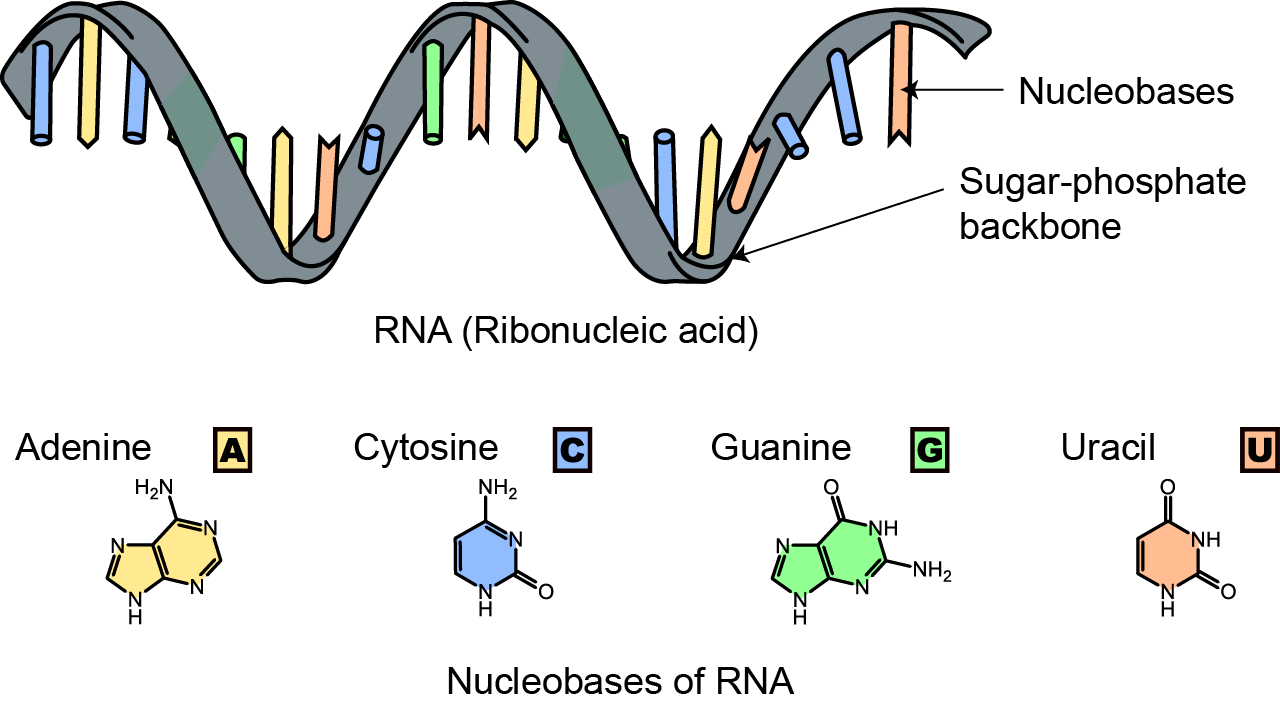
\includegraphics[width=0.5\textwidth]{fig01/rna_bases.png}
  \caption{Single strand RNA \newline (modified from the original version by \href{https://commons.wikimedia.org/w/index.php?curid=9810855}{Sponk, Wikimedia Commons})}
\end{figure}

\noindent \textbf{Transcription: mRNAs are transcribed from DNAs}

\begin{verbatim}
DNA: ACGT -------> RNA: ACGU
        Transcription
\end{verbatim}

%
% Protein
%
\subsubsection*{Protein}

Proteins are large molecules consisting of amino acids. There are 20 common amino acids.
 
\begin{figure}[H]
  \centering
      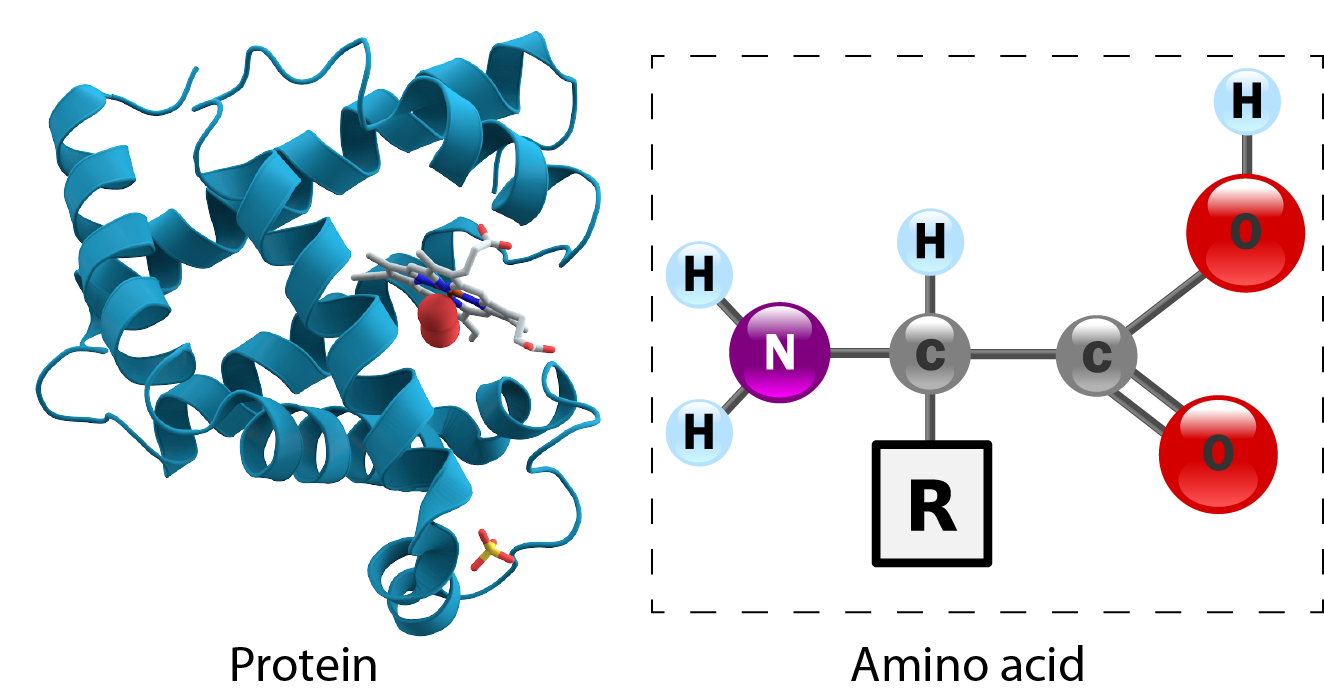
\includegraphics[width=0.6\textwidth]{fig01/protein_and_amino_acid.png}
  \caption{Protein 3D structure and amino acids \newline (sources: \href{https://en.wikipedia.org/wiki/Protein\#/media/File:Myoglobin.png}{AzaToth, Wikimedia Commons}, \href{https://en.wikipedia.org/wiki/Amino_acid\#/media/File:AminoAcidball.svg}{YassineMrabet, Wikimedia Commons})}
\end{figure}

\noindent \textbf{Translation: Amino-acids are translated from mRNAs}

\begin{verbatim}
mRNA: GUC -------> AA: Valine
        Translation
\end{verbatim}

\newpage 

\noindent \textbf{Universal genetic code}

\noindent A codon consists of three nucleic acids. Single-letter or three-letter names can be used for amino acids.

\begin{figure}[H]
  \centering
      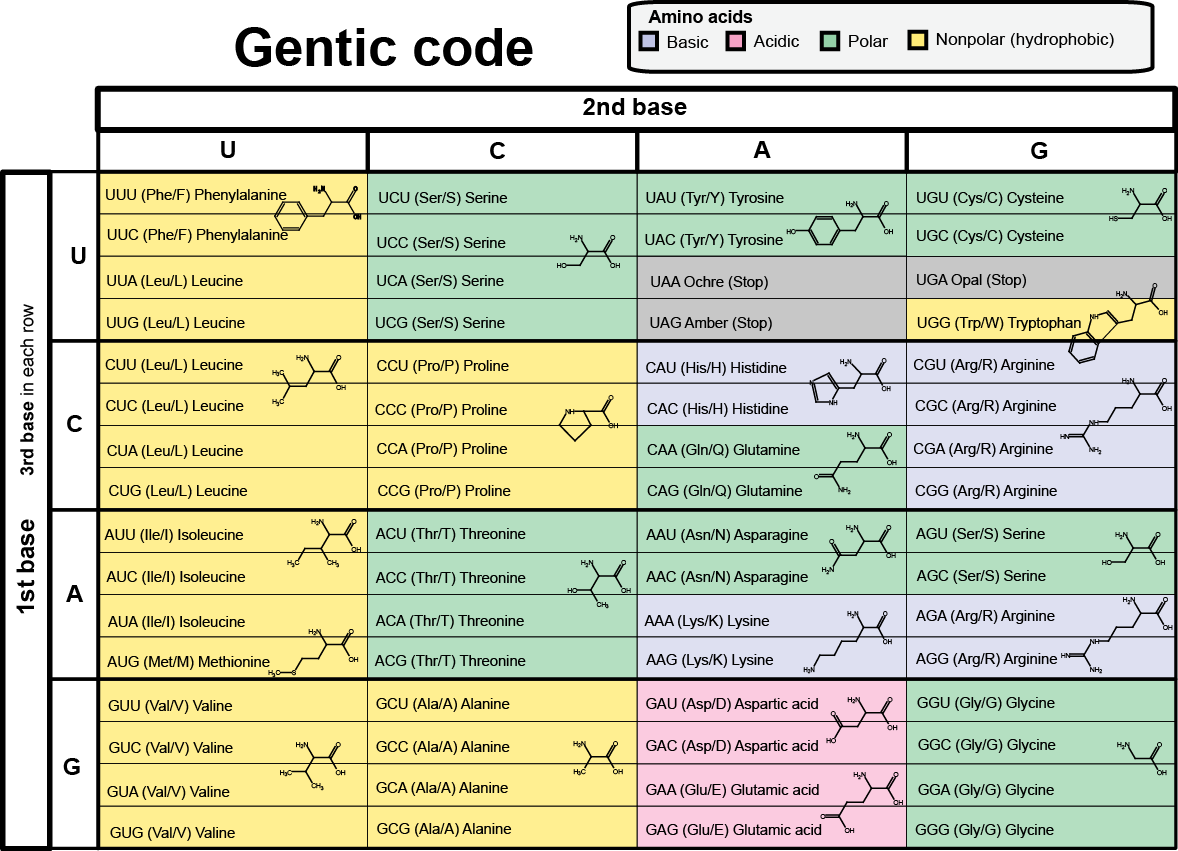
\includegraphics[width=0.7\textwidth]{fig01/genetic_code.png}
  \caption{Universal genetic code \newline (modified from the original version by \href{https://commons.wikimedia.org/wiki/File\%3ANotable_mutations.svg}{H\"aggstr\"om, Wikimedia Commons})}
\end{figure}

\noindent \textbf{Cellular functions of proteins}
\begin{itemize}
\item Enzymes: catalyze chemical reaction
\item Cell signaling: hormone (e.g. insulin), antibodies, …
\item Structural: collagen, cartilage, keratin, …
\end{itemize}

%
% Exercises 1.1
%
\subsubsection*{Exercises 1.1}
\begin{enumerate}

\item Draw a simple diagram of the central dogma of molecular biology and briefly explain the information flow of the molecules.

\item What are the DNA sequences of the opposite strand for the following DNA sequences?
\begin{verbatim}
    Seq1 CCGATT
    Seq2 TTACGC
    Seq3 ACGCGC
\end{verbatim}

\item What are the mRNA sequences transcribed from the following DNA sequences?

\item What are the polypeptide sequences translated from the following mRNA sequences? Answer them with both one-letter and three letter names.
\begin{verbatim}
    Seq1 AUGUUUUAA
    Seq2 GCAGCAAAA
\end{verbatim}
		
\end{enumerate}

%\end{document}

%\documentclass[12pt]{article}
%\usepackage[a4paper, margin=1in]{geometry} 
%\usepackage{graphicx} 
%\usepackage{hyperref}
%\usepackage{float}
%\usepackage[font=small, labelfont=bf]{caption}

%\begin{document}

%
% Introduction to Biotechnology
%
\subsection{Introduction to Biotechnology}
Biotechnology is the use of laboratory techniques to study living organism and cells. 

%
% Applications of biotechnology
%
\subsubsection*{Applications of biotechnology}
Branches of biotechnology can be explained with different colors.
\begin{itemize}
\item Red: medical processes
\item Green: agricultural processes
\item White: industrial processes
\item Blue: marine and aquatic applications
\end{itemize}

%
% Laboratory tools and equipment
%
\subsubsection*{Laboratory tools and equipment}

\begin{figure}[H]
  \centering
      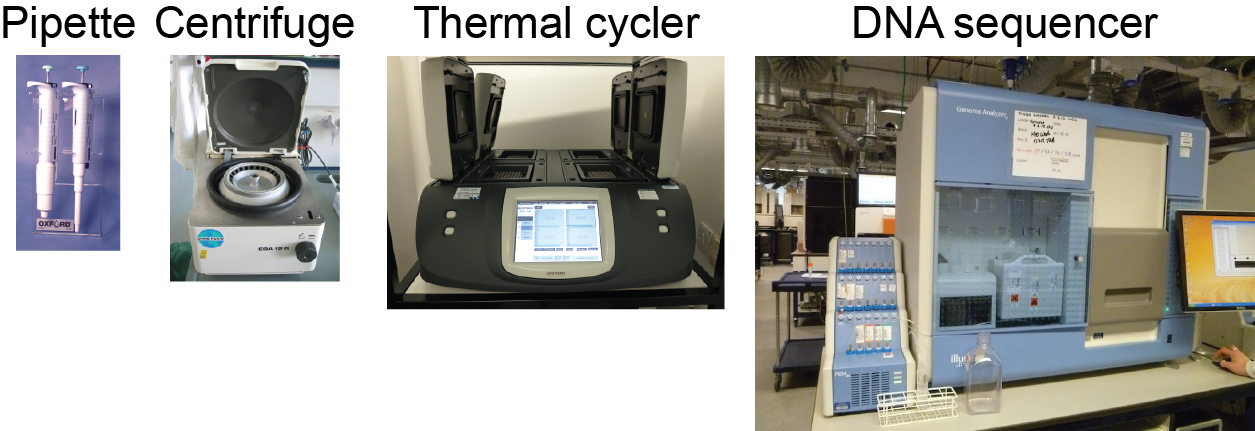
\includegraphics[width=0.5\textwidth]{fig01/lab_equipment.png}
  \caption{Pipette, centrifuge, thermal cycler, and DNA sequencer \newline (sources:  \href{https://en.wikipedia.org/wiki/Pipette\#/media/File:Single_channel_rack.jpg}{Domain}, \href{https://commons.wikimedia.org/w/index.php?curid=494}{Manske},
\href{https://commons.wikimedia.org/w/index.php?curid=20189025}{Rror}, 
\href{https://commons.wikimedia.org/w/index.php?curid=18862968}{RE73} via Wikimedia Commons)}
\end{figure}
 
%
% Human genome project
%
\subsubsection*{Human genome project}
It was a large-scale international research project to determine the whole DNA sequences of human.

\begin{itemize}
\item 1990 –- 2003
\item \$2.7 billion
\end{itemize}

%
% Next generation sequencing
%
\subsubsection*{Next generation sequencing}
Sequence technologies have been rapidly advanced since the human genome project.

Example: sequence a whole human genome with Illumina HiSeq X Ten.
\begin{itemize}
\item One day
\item \$1000
\end{itemize}

%
% Protein sequencing
%
\subsubsection*{Protein sequencing}
Proteins are generally more studied than DNAs and RNAs, but the whole proteome is generally harder to analyze than the whole genome. MS (mass-spectrometry) based technologies are widely used to sequence proteins.

\begin{figure}[H]
  \centering
      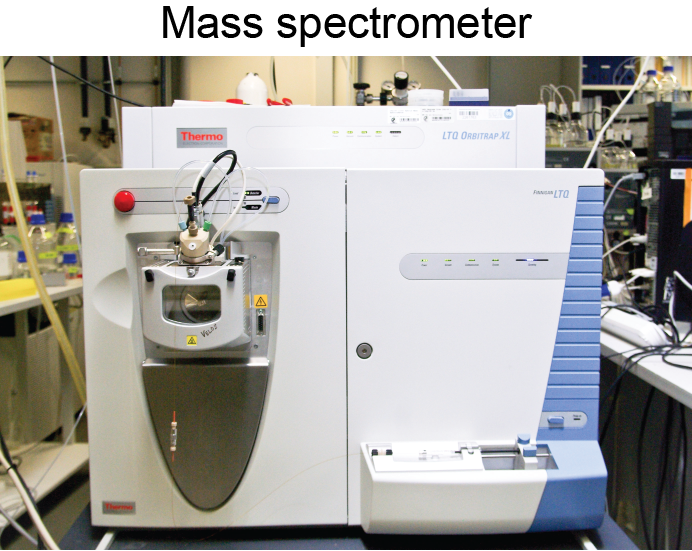
\includegraphics[width=0.25\textwidth]{fig01/mass_spectrometer.png}
  \caption{Orbitrap mass spectrometer (source: \href{https://commons.wikimedia.org/w/index.php?curid=18691799}{Wi\`{o}rkiewicz, Wikimedia Commons})}
\end{figure}
 
%\end{document}


\end{document}


